\chapter{A Systematic Mapping Study on Game-related Methods for Software Engineering Education}
\label{ch:sms}

The goal of this chapter is to identify and discuss game-related methods in the context of software engineering education. We call game-related methods for software engineering education, any approach where games are used to support the process of teaching or learning software engineering. Therefore, we conducted a systematic mapping study to survey the software engineering education literature in order to: (i) identify game-related methods for software engineering education; (ii) understand how these game-related methods support the software engineering knowledge areas from SE 2014; and (iii) understand specific characteristics of each game-related method. 

Previous studies \citep{Marques:2014, Malik:2012, Caulfield:2011, Kosa:2016} investigated and mapped educational methods in the software engineering education context. This study complements previous ones by providing the following novel contributions to the community. First, we propose a classification scheme for game-related educational methods used in software engineering education. Second, we analyze the difference in the proposal and application of methods found in the literature. Third, we also discuss how these educational methods support specific software engineering education knowledge areas.

From the 156 primary studies analyzed, we identified three game-related methods used in software engineering education: “Game-based Learning”, “Game Development Based Learning”, and “Gamification”. We mapped their learning goals and identified that these educational methods are mostly used to support the knowledge areas of “Software Process”, “Software Design” and “Professional Practice” (as described in \cite{Acm:2015}). However, each educational method has different purposes and rationales to support these knowledge areas, thus serious games are more used in the context of “Software Process” education, while “Game Development Based Learning” is more used in “Software Design” education. Gamification in software engineering education is new, and initial results are promising, however, further investigation and additional empirical evidences are still needed for the discussion of its effectiveness in this context.

The remainder of this chapter is organized as follows. Section 2 provides the necessary theoretical foundation for the study. In Section \ref{sec:smsstudySettings}, we describe the design of this systematic mapping study. Section \ref{sec:smsresults} presents the results of the study and Section \ref{sec:smsdiscussion} discusses the results and provides insights about the role of each game related method in software engineering education. In Section \ref{sec:smsthreats}, we discuss the threats to the validity of the study. Section \ref{sec:final} concludes this research paper.

\section{Study Settings}
\label{sec:smsstudySettings}

This section presents the goals of this study and the methodology adopted. Section \ref{sec:smsgoals} presents the study goal and research questions. Section \ref{sec:smsmethod} explains the research method and the process executed. Section \ref{sec:smssearch} discusses the search strategy applied to mine relevant scientific databases. Section \ref{sec:smsselection} shows the selection process filtering only relevant papers for this study. Section \ref{sec:smsdataextraction} presents the classification scheme and mapping strategy used to present the study results.

\subsection{Goal and research questions}
\label{sec:smsgoals}

The goal of this study is to identify and analyze game-related methods from the purpose of understanding their application and learning objectives in the context of software engineering education. To achieve this goal, we established five research questions:

\textbf{RQ1.} What game related methods have been proposed for supporting software engineering education?

\textbf{RQ2.} What software engineering education knowledge areas are supported by the existing game-related methods?

\textbf{RQ3.} What game elements have been used for the Gamification of software engineering education? 

Based on the classification scheme for game-related methods for software engineering education [5], the expected outcome of RQ1 is a list of primary studies categorized by approach type. The expected outcome of RQ2 is a mapping between learning objectives from the approaches identified in RQ1 and the software engineering knowledge areas from SE 2014. Finally, the expected outcome of RQ5 is a summary of game elements, mechanics, and dynamics extracted from the list of Gamification approaches identified in RQ1.

\subsection{Method}
\label{sec:smsmethod}

To achieve the study goal, we have conducted a Systematic Mapping Study (SMS). SMS is a secondary study method that systematically (i.e., based on a structured and repeatable process or protocol) explores and categorizes studies in a given research field, and provides a structure of the type of research reports and results that have been published \citep{Petersen:2007}[20]. SMS results are often organized as visual summaries (maps). The expected contribution is to provide researchers and educators with an overview of the state-of-the-art on the use of games and game elements for supporting software engineering knowledge areas from the educational perspective. Additionally, we expect to identify possible research gaps and trends.

We have conducted the SMS in the period of June/2016 to December/2016, following four process steps adapted from Petersen et al. \citep{Petersen:2007} (Figure \ref{fig:smsprocess}).

\begin{figure}[!h]%th
\centering
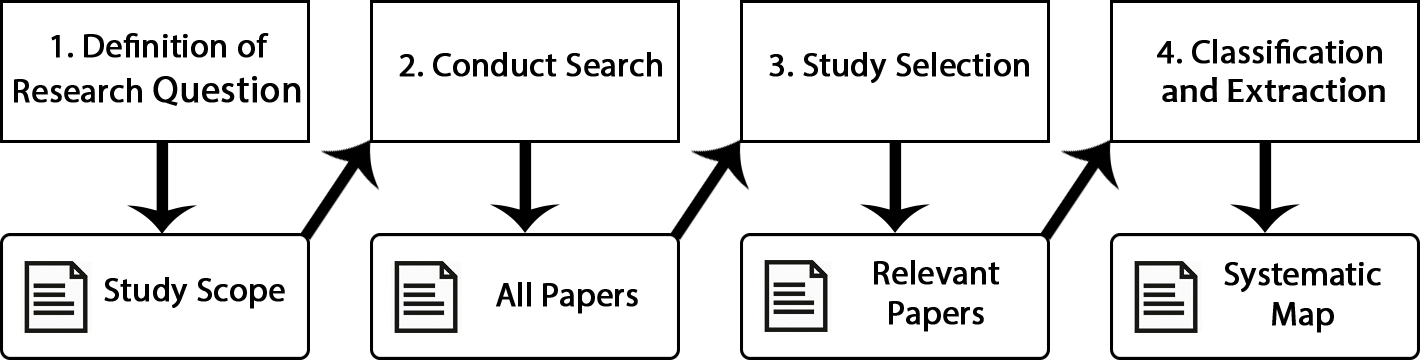
\includegraphics[width=0.8\textwidth]{img/smsprocess.png}
\caption{Systematic mapping process, adapted from \cite{Petersen:2007}}
\label{fig:smsprocess}
\end{figure} 

\textbf{Step 1} – Definition of research questions: We have defined five research questions based on the study goal, to establish the desired scope of the systematic study (Section \ref{sec:smsgoals});

\textbf{Step 2} – Conduct search: based on the research questions, we defined and performed a replicable process for searching for retrieving papers in selected scientific databases (Section \ref{sec:smssearch});

\textbf{Step 3} – Study Selection: We have defined and applied a replicable process for selecting only the relevant papers for this study (Section \ref{sec:smsselection});

\textbf{Step 4} – Study Classification and Data Extraction: Based on the research questions, we have defined a strategy for mapping the relevant data from the primary studies (Section \ref{sec:smsdataextraction}) and for presenting the study results (Section \ref{sec:smsresults}). 

Five researchers participated in the planning and execution of the study: an undergraduate student in CS, a PhD student in CS, and three PhD associate professors teaching software engineering courses in two different institutions.

\subsection{Search strategy}
\label{sec:smssearch}

The search strategy enables the inclusion of relevant studies in the search results. To identify possible primary studies for data extraction, the search was based on (i) trial searches using combinations of keywords derived from the study goal for the definition of valid search strings and (ii) the execution of automatic searches in the scientific databases using the search strings. 	Initially, we selected relevant keywords related to the three domains under analysis: (a) education; (b) software engineering; and (c) game-related approaches. In order to identify these relevant keywords, we considered search strings used in related systematic studies, bodies of knowledge and curricula guidelines for software engineering, and experts (software engineering educators). The resulting keywords per domain were:

\textbf{Education:} teach, learn, education, train;

\textbf{Software engineering:} software engineering, software process, software requirements, requirements engineering, software verification, software validation, software design, software architecture, software test, software quality, software project management;

\textbf{Game-related approaches:} game, serious games, edutainment, gamification, game based learning, gbl.

Search strings were defined by grouping keywords in the same domain with the logic operator “OR” and grouping the three domains with the logic operator “AND”. We then executed automatic searches in four selected scientific databases, using and adapting (when necessary) the search string. The databases used were ACM Digital Library , IEEE Xplore , EI Compendex , and Scopus , since they have a large amount of relevant conferences and journals indexed. We limited the results of automatic searches to return only papers written in English, and we did not apply any time limitation.

\subsection{Study selection}
\label{sec:smsselection}

In this step, we filtered the studies retrieved from the automatic searches by some steps to exclude papers not aligned with the study goals. First, the five researchers defined the following inclusion and exclusion criteria:

•	Inclusion Criteria: Studies whose main focus was on proposal, usage, discussion or evaluation of game-related methods in the context of software engineering education;

•	Exclusion Criteria: Papers not written in English; Papers not fully available to download; Studies formatted as short papers (2 or less pages), tutorials, demos, books, book chapters, and similar; secondary studies; and duplicated studies.

The study selection process was executed in two phases: (i) in the first selection phase, two researchers individually read all titles and abstracts and removed studies that did not comply with inclusion criteria; (ii) in the second selection phase, they have downloaded all remaining papers and each researcher examined all papers’ introduction and conclusion to remove studies that matched the exclusion criteria. During these steps, any conflict was solved with a third researcher. For any persisting problem, the two remaining researchers were consulted for a final decision regarding the inclusion or exclusion of a primary study. However, only a few conflicts emerged in the first selection phase (less than 7\% of the selected studies), and most cases because the learning topic was not clearly related to software engineering. In the second selection phase, those conflicted studies were carefully read and the third researcher helped in the decision of inclusion or exclusion. Therefore, we believe the selection process is clear and precise enough for replication.

Table \ref{table:studyseleciton} summarizes the result of the selection process. The first column (Source) presents the scientific databases mined and the second one (\# Papers) describes the number of papers retrieved from the use of the search strings. The third (1st Selection) and fourth (2nd Selection) columns shows the number of remaining papers after the execution of the first and second selection phases, respectively. The fifth column (\% Included) describes the ratio between the remaining papers after the selection process (2nd Selection) and the total number of papers retrieved from each database (\# Papers). Finally, the last column (Interval) presents the time range of the resulting primary studies.


\begin{table}[htb]
\caption{Results of the study selection process}
\label{table:studyseleciton}
\centering
\newcolumntype{Y}{>{\centering\arraybackslash}X}
\scriptsize
\begin{tabularx}{\textwidth}{>{\hsize=.35\hsize}X>{\hsize=.3\hsize}Y>{\hsize=.35\hsize}Y>{\hsize=.35\hsize}Y>{\hsize=.3\hsize}Y>{\hsize=.3\hsize}Y}
\hline
\textbf{Source} & \textbf{\# Papers} & \textbf{1st Selection} & \textbf{2nd Selection} & \textbf{\% Included} & \textbf{Interval}  \\ \hline
ACM DL       & 1204      & 248           & 42            & 3,49\%      & 1974-2016 \\
IEEE Xplore  & 558       & 155           & 69            & 12,37\%     & 1977-2015 \\
EI Compendex & 1133      & 313           & 120           & 10,68\%     & 1982-2016 \\
Scopus       & 1270      & 336           & 132           & 10,47\%     & 1974-2016 \\
Total        & 4165      & 1052          & 363           & 8,72\%      & 1974-2016 \\
Total*       & 2675      & 568           & 156           & 5,83\%      & 1974-2016 \\
\hline
\end{tabularx}
\end{table}

The study selection process resulted in 156 unique primary studies. However, we found a high number of duplicates among different scientific databases. Figure \ref{fig:smsdistribution} illustrates the overlapping results between databases. We removed the duplicated papers from the results of the automatic search (\# Papers). However, for the purpose of documentation and analysis, we kept track of the database from where each paper was found. 

\begin{figure}[!h]%th
\centering
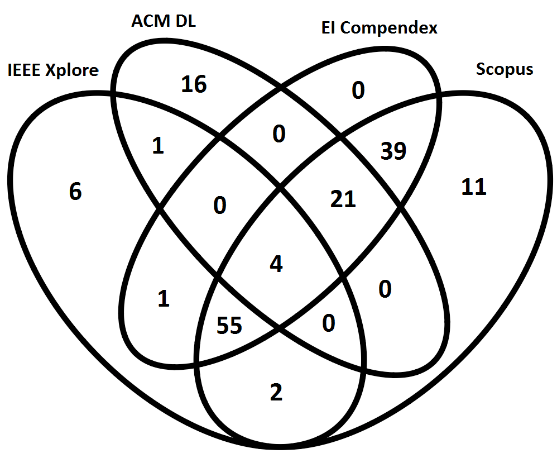
\includegraphics{img/smsDistribution.png}
\caption{Distribution of Primary Studies per Database.}
\label{fig:smsdistribution}
\end{figure} 

\subsection{Study classification and data extraction}
\label{sec:smsdataextraction}

We analyzed the resulting list of primary studies for extracting information by identifying: (i) the presented approach; (ii) the game-related method used; and (iii) learning objectives or expected developed skills. We classified each approach using game-related methods (RQ1) in the following categories [5]: Gamification, GBL, and GDBL (as described in Section 2.2). 	We then identified the expected learning outcomes and mapped them to the purpose and related topics of the knowledge areas from SE 2014. 

\section{Results}
\label{sec:smsresults}

In this section, we presented the results of the systematic mapping study. Section \ref{sec:smsresultoverview} provides an overview of the primary studies selected for this study. Sections \ref{sec:smsrq1} to \ref{sec:smsrq3} describes the results for the research questions RQ1 to RQ3, respectively.

\subsection{Overview}
\label{sec:smsresultoverview}

The study selection resulted in 156 primary studies, published between 1974 to June 2016. Figure \ref{fig:smstimeline} presents a histogram with the frequency of primary studies per year, with different colors representing the types of approaches found (discussed in details in Subsection \ref{sec:smsrq1}). This result suggests that software engineering education has been a challenge since the early years of software engineering in the 1970’s, and that the use of game-related educational methods is not a novelty. Nonetheless, since 2002 there has been a constant and growing presence of studies about the use of game-related methods for software engineering education.

\begin{figure}[!h]%th
\centering
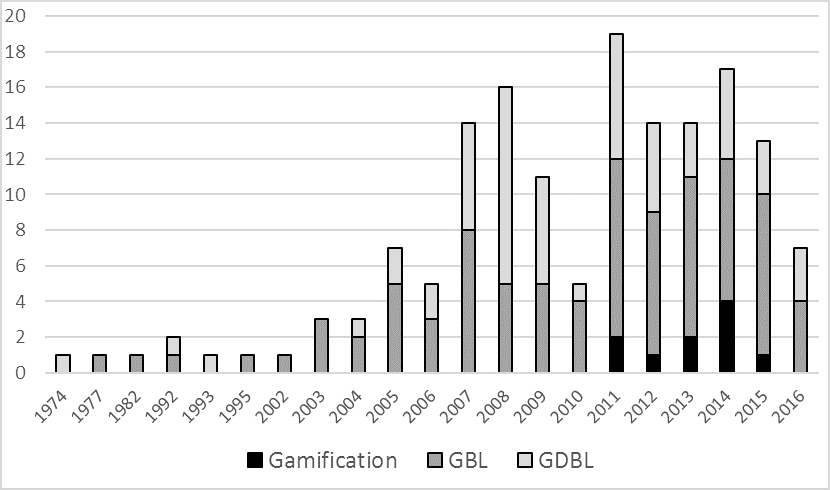
\includegraphics{img/smsTimeline.png}
\caption{Timeline of primary studies.}
\label{fig:smstimeline}
\end{figure} 

Figure \ref{fig:smsforum} shows the distribution of studies per type of forum. The majority of the primary studies was published in conferences (69\%), but we also retrieved studies from journals (24\%) and workshops (7\%). The conferences with greater occurrences of primary studies were CSEE&T, FIE, SIGCSE, and ICSE. Table \ref{table:publicationvenues} summarizes the most recurring publication venues in our study and their respective counting of selected primary studies. We list the publication venues that have three or more primary studies selected in this study. Appendix A provides the complete list of primary studies. In the remainder of this paper, we used unique identifications (PS<number>) when referring to primary studies.

\begin{figure}[!h]%th
\centering
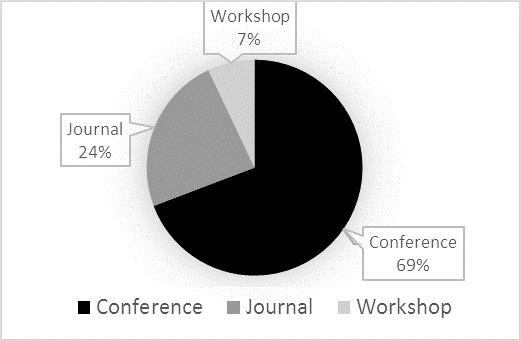
\includegraphics{img/smsForum.png}
\caption{Distribution of primary studies per type of forum.}
\label{fig:smsforum}
\end{figure} 

\begin{table}[htb]
\caption{Relevant publication venues for game related approaches in software engineering education}
\label{table:publicationvenues}
\centering
\newcolumntype{Y}{>{\centering\arraybackslash}X}
\scriptsize
\begin{tabularx}{\textwidth}{>{\hsize=.15\hsize}Y>{\hsize=.8\hsize}X}
\hline

\textbf{\# Studies} & \textbf{Publication Venues}                                                       \\
15         & IEEE Conference on Software Engineering Education and Training (CSEE\&T) \\
13         & Frontiers In Education Conference (FIE)                                  \\
11         & ACM Technical Symposium on Computer Science Education (SIGCSE)           \\
10         & International Conference on Software Engineering (ICSE)                  \\
5          & Journal of Computing Sciences in Colleges                                \\
4          & IEEE Transactions on Education                                           \\
4          & IEEE Global Engineering Education Conference (EDUCON)                    \\
3          & International Conference on Computer Games (CGAMES)                      \\
3          & International Workshop on Games and Software Engineering (GAS)           \\
3          & International Journal of Computer Games Technology                       \\
3          & ASEE Annual Conference and Exposition         \\            

\hline
\end{tabularx}
\end{table}

\subsection{RQ1 – Game-related methods for software engineering education}
\label{sec:smsrq1}

This section discusses the results for the first research question  \textit{RQ1. "What game-related methods have been proposed to support software engineering education?"}.

In accordance to the classification described in Section 3.5, 88 primary studies presented the use of GBL method, 60 presented the use of GDBL method, and 11 presented Gamification approaches. Three primary studies presented hybrid approaches, i.e., the combination of two distinct methods: (i) one used Gamification and GDBL; and (ii) two used GDBL and GBL. Table \ref{table:smscategories} presents the mapping of game-related methods found (Method), the primary studies that use each method (Primary Studies) and their quantity, and the number of studies that have some sorts of evaluation in the classroom.
 
\begin{table}[htb]
\caption{Mapping of categories of game-related methods and primary studies}
\label{table:smscategories}
\centering
\newcolumntype{Y}{>{\centering\arraybackslash}X}
\scriptsize
\begin{tabularx}{\textwidth}{>{\hsize=.3\hsize}X>{\hsize=.25\hsize}Y>{\hsize=.25\hsize}Y>{\hsize=.25\hsize}Y}
\hline
\textbf{Method}       & \textbf{Primary Studies} & \textbf{\# Primary Studies} & \textbf{Evaluation} \\ \hline
Gamification          & PS001 - PS010            & 10 (6.4\%)  & 6 (60\%)            \\
GBL                   & PS011 - PS096            & 86 (55.1\%) & 45 (52,3\%)         \\
GDBL                  & PS097 - PS153            & 57 (36.5\%) & 18 (31,6\%)         \\
Gamification and GDBL & PS154                    & 1 (0.6\%)     & 0                   \\
GBL and GDBL          & PS155 - PS156            & 2 (1.2\%)   & 1 (50\%)       \\    
\hline
\end{tabularx}
\end{table}

GBL and GDBL are the most prevalent methods found in this study. Both methods are used to support software engineering education since the decade of 1970’s (PS082, PS143). GBL approaches include serious games and non-serious games in digital or non-digital formats. Some examples of serious games include GetKanban (PS087), PMG-2D (PS071), and InspectorX (PS055), designed to support the learning of Kanban, project management and software inspection, respectively. The use of games as learning tools (GBL approaches) is usually motivated by the opportunity of teaching learning topics difficult to explore in traditional lectures. This difficulty is often caused by limitations imposed by the nature of the topic, by time restrictions of traditional lectures or by practical problems related to real life experiences hard to translate to examples in the classroom. For instance, Smart Decisions (PS080) is a game developed to aid in teaching architecture design. \cite{Cervantes:2016} suggest “software architecture courses frequently rely on relatively simple examples (…) Such examples may present the essential concepts of design, but they are also distant from real life system design experiences”. The authors also suggest that the timeframe is too short to observe consequences of the decisions that are made as part of the design process \citep{Cervantes:2016}. Therefore, games are useful to support the setup of a controlled environment that can simulate real life experiences. 

Primary studies proposing the use of GDBL method are divided in two types: (i) assignments on developing game products; and (ii) adoption of game development frameworks. The former studies describe experiences of students’ assignment with hands-on experience in the domain of game development to introduce the challenges of software engineering. For instance, PS111 describes and evaluates a block course in which students with almost no mobile application development experience create games in just two weeks. These students learn modeling, design patterns, software configuration management, and game development. PS123 employs game “play testing” for learning about issues and challenges of modern software engineering projects and practices. The later studies advocate the use of game development frameworks as learning instruments to simplify certain aspects of development (e.g., technicalities of learning a new language) and allowing students to concentrate efforts on specific learning goals (e.g. software design). For instance, PS150 describes a case study of how a game project using the XNA Game Studio from Microsoft was implemented in a software architecture course.

Concerning Gamification, although the term is recent in literature \citep{Deterding:2011}, it was rapidly incorporated in software engineering education since 2011 (PS007, PS010). Gamification approaches found are usually applied as an innovative learning context more focused in engaging and motivating learners to perform desired behaviors. However, we observed two different strategies for the use of Gamification in software engineering education: (i) Gamification of the classroom experience and (ii) Gamification of specific software engineering activities. Gamification of the classroom experience refers to the use of game elements to engage and motivate students in performing learning activities (PS003, PS004, PS005, PS008). For instance, PS005 describes the experiment of implementing Gamification techniques into software engineering and service-oriented architecture courses using Points, Leaderboards and Badges to promote competition and, consequently, to motivate students in the class activities. The strategy is focused in the Gamification of the classroom activities, and not specific software engineering related activities. 

Gamification of specific software engineering activities, on the other hand, applies game elements to motivate learners in practicing specific skills or performing specific practices (PS001, PS002, PS006, PS007, PS010). PS006 describes an experiment in which students are encouraged to make more frequent commits to version control system, in a software project course. The authors proposed a leaderboard based on the number of commits from each student, and established milestones/thresholds that would trigger messages congratulating students and teams that reached the specified number of commits. PS01 uses weekly challenges to motivate students on applying eXtreme Programming practices to their project. In this scenario, students compete for a “challenge cup” award.

Some studies (PS154, PS155, and PS156) mix the previous approaches in order to achieve better learning results (hybrid approaches). Two studies (PS155 and PS156) discuss the advantages of learning cycles where students play and develop serious games. One study (PS154) proposes a hybrid approach consisting of developing games focusing on good design, and applying a gamified strategy for testing it.

Regarding the evaluation of those studies, most of them adopt case studies or pilot studies in classroom. However, only 70 primary studies formally describe proper evaluation methods and results, regarding effectiveness in learning or perception of users: 45 (out of 86 – 52,3\%) studies on GBL method; 18 (out of 57 – 31,6\%) studies on GDBL method; 6 (out of 10 – 60\%) on Gamification; and 1 (out of 3 – 33,3\%) on hybrid approaches. The most recurring evaluation strategies rely on pre-test and post-test, and on questionnaires. The higher number of GBL studies with proper evaluation, in comparison to GDBL, may relate to the nature of GBL approaches: The evaluation of serious games can be performed in shorter periods, while the evaluation of development project requires longer periods. Consequently, this factor may impact on availability of participants and in the effort to perform comparative studies with control groups. In the case of Gamification, the total number of primary studies is low, therefore further investigation and additional empirical evidences are still needed for the discussion of its effectiveness in software engineering education.

\subsection{RQ2 - Mapping learning goals to SE 2014 Knowledge Areas}
\label{sec:smsrq2}

This section discusses the results for the following research question.

\textit{RQ2. What software engineering education knowledge areas are supported by the existing game-related approaches?}

We identified the learning goals of each primary study and mapped them to the SE 2014 knowledge areas (KA) described in Section 2.1 (Table \ref{table:kamap}). The results show that “Software Process” is the KA with the greater number of primary studies with game related approaches supporting it (92 - 59\%), followed by “Software Design” (60 – 38.5\%), “Professional Practice” (48 – 30.8\%), “Requirement Analysis and Specification” (39 – 24.3\%), and “Software Verification and Validation” (30 – 19.2\%). The least supported KA are “Software Quality” (10 – 6.4\%) and “Software Modelling and Analysis” (10 – 6.4\%).

\begin{table}[htb]
\caption{Mapping of knowledge areas (KA) from SE 2014 and Primary Studies}
\label{table:kamap}
\centering
\newcolumntype{Y}{>{\centering\arraybackslash}X}
\scriptsize
\begin{tabularx}{\textwidth}{>{\hsize=.1\hsize}Y>{\hsize=.75\hsize}X>{\hsize=.15\hsize}Y}
\hline
\multicolumn{1}{c}{\textbf{K.A.}} & \multicolumn{1}{c}{\textbf{Primary Studies}} & \multicolumn{1}{c}{\textbf{\#}} \\ \hline
PRO & PS001; PS002; PS006; PS007; PS011; PS012; PS014; PS015; PS016; PS017; PS019; PS020; PS021; PS022; PS023; PS025; PS026; PS027; PS028; PS029; PS030; PS034; PS035; PS036; PS037; PS039; PS040; PS042; PS043; PS044; PS045; PS046; PS049; PS050; PS052; PS054; PS057; PS058; PS059; PS060; PS061; PS062; PS063; PS064; PS068; PS069; PS070; PS071; PS074; PS075; PS076; PS077; PS079; PS081; PS084; PS086; PS087; PS088; PS089; PS091; PS092; PS094; PS096; PS097; PS102; PS107; PS110; PS111; PS115; PS116; PS118; PS119; PS120; PS121; PS122; PS124; PS128; PS129; PS130; PS131; PS134; PS135; PS140; PS141; PS142; PS144; PS145; PS146; PS148; PS151; PS155; PS156; & 92 (59\%)                       \\
DES & PS007; PS015; PS020; PS026; PS048; PS056; PS065; PS073; PS080; PS081; PS089; PS095; PS097; PS098; PS099; PS100; PS101; PS103; PS105; PS107; PS108; PS110; PS111; PS112; PS113; PS114; PS116; PS117; PS119; PS120; PS121; PS122; PS123; PS124; PS125; PS126; PS127; PS129; PS130; PS132; PS133; PS134; PS135; PS136; PS137; PS138; PS139; PS140; PS142; PS143; PS144; PS145; PS146; PS148; PS149; PS150; PS152; PS153; PS154; PS155;  & 60 (38.5\%)                     \\
PRF & PS007; PS012; PS013; PS014; PS015; PS017; PS018; PS020; PS025; PS026; PS030; PS031; PS043; PS061; PS064; PS072; PS081; PS085; PS086; PS090; PS091; PS097; PS099; PS102; PS106; PS107; PS110; PS111; PS119; PS121; PS124; PS128; PS129; PS130; PS134; PS135; PS139; PS141; PS143; PS144; PS145; PS146; PS147; PS148; PS151; PS152; PS155; PS156; & 48 (30.8\%)                     \\
REQ & PS007; PS013; PS014; PS015; PS017; PS020; PS026; PS032; PS043; PS047; PS048; PS051; PS053; PS078; PS090; PS093; PS097; PS101; PS107; PS110; PS114; PS116; PS117; PS119; PS120; PS121; PS122; PS123; PS124; PS128; PS129; PS130; PS134; PS140; PS142; PS145; PS146; PS148; PS155; & 39 (24.3\%)                     \\
VAV & PS007; PS010; PS015; PS024; PS033; PS038; PS048; PS055; PS066; PS067; PS083; PS107; PS109; PS114; PS116; PS119; PS120; PS121; PS122; PS123; PS129; PS134; PS142; PS144; PS145; PS146; PS148; PS152; PS154; PS155;  & 30 (19.2\%)                     \\
MAA & PS007; PS116; PS120; PS131; PS134; PS138; PS140; PS142; PS148; PS152; & 10 (6.4\%) \\
QUA & PS007; PS014; PS058; PS097; PS110; PS116; PS129; PS140; PS142; PS148; & 10 (6.4\%)                   \\
\hline
\end{tabularx}
\end{table}

The KA “Software Design” (DES), “Requirement Analysis and Specification” (REQ) and “Software Verification and Validation” (VAV) are directly linked to recurrent phases in software development lifecycle models (e.g., the phases of “Requirements”, “Design” and “Verification” in representations of the waterfall model). Consequently, the primary studies proposed learning experiences that address each of these KA specifically or setups where students experience topics related to these KA in the context of a software development process. 	Most of the primary studies mapped to the KA “Professional Practice” proposes game related approaches that directly support other KA and, as secondary goal, they encourage the development of professional or “soft” skills. These skills are usually related to dynamics of working in teams or groups, interacting with stakeholders, communication, and leadership.

We found few primary studies indicating the support for KA “Software Quality” (QUA) and “Software Modeling and Analysis” (MAA). Usually, the supporting for MAA was related to applying UML (Unified Modeling Language) in software design for documentation and analysis purposes. The supporting for QUA was related to definition and appliance of quality assurance procedures in the contexts of software process and software verification. The description of these knowledge areas \citep{Acm:2015} reflects their “supportive” nature: (i) MAA is described as “essential to documenting and evaluating design decisions and alternatives”; and (ii) QUA is described as a “crosscutting concern” and is suggested that “software quality topics must be integrated into the presentation and application of material associated with other KA”. 

Regarding the support of Knowledge Areas by each game-related method, Figure \ref{fig:smsbubble} describes a quantitative relationship between game-related methods and the coverage of each SE 2014 knowledge area. The different nature of each game-related method results in different strategies to support learning goals. The GBL approaches usually focus on few learning topics: 65 out of 88 (73.9 \%) primary studies describing GBL approaches support only one knowledge area. In contrast, 23 out of 60 (38.3 \%) primary studies describing GDBL approaches support a single knowledge area. This analysis shows that GBL approaches are, usually more specific in terms of learning goals, while the practical nature of GDBL approaches are broader.

\begin{figure}[!h]%th
\centering
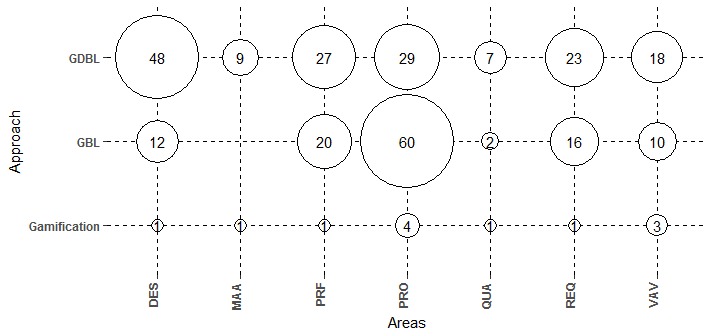
\includegraphics[width = 1\textwidth]{img/smsBubble.png}
\caption{Distribution of primary studies per type of forum.}
\label{fig:smsbubble}
\end{figure}

The mapping of Figure \ref{fig:smsbubble} also shows that “Software Design” (DES) is predominant in GDBL approaches, while “Software Process” (PRO) is predominant in GBL approaches. We observed that GDBL method favors hands-on experience on software design in a domain of systems familiar to students. The use of game development frameworks helps overcoming technology barriers (e.g. complexity of learning new programming languages) in software development, allowing students to focus on learning good design. This practical nature of GDBL approaches also reflects the higher number of primary studies supporting “Software Quality” (QUA) and “Software Modeling and Analysis” (MAA), providing learners with the experience of learning by doing.

The challenges and nuances of software process are difficult to simulate in student projects because of diverse factors (e.g., limitation of time, limitation of students’ availability). Therefore, games and simulations play a great role in creating abstractions and simplifications of real life software development.

\subsection{RQ3 - Gamification elements used in software engineering education}
\label{sec:smsrq3}

This section discusses the results for the last research question.

\textit{RQ3. What game elements have been used for the Gamification of software engineering education?}

In order to understand how Gamification is being used in the context of software engineering education, we analyzed which game elements are used in each primary study (Table \ref{table:smsgamification}). Leaderboards, Points, and Levels are the recurrent game mechanics found (5, 4, and 4 primary studies, respectively). Competition is the most recurring game design principle identified (4 primary studies).

\begin{table}[htb]
\caption{Game elements identified in primary studies}
\label{table:smsgamification}
\centering
\newcolumntype{Y}{>{\centering\arraybackslash}X}
\scriptsize
\begin{tabularx}{.8\textwidth}{>{\hsize=.5\hsize}X>{\hsize=.5\hsize}X}
\hline
\multicolumn{1}{c}{\textbf{Game Element}} & \multicolumn{1}{c}{\textbf{Primary Studies}} \\ \hline
Leaderboards                              & PS003, PS002, PS005, PS007, PS006            \\
Points                                    & PS010, PS003, PS002, PS005, PS154            \\
Milestones, Levels, Paths and Progress    & PS010, PS003, PS007, PS006, PS154            \\
Competition                               & PS001, PS003, PS005, PS007                   \\
Collaboration, Altruism, Teams            & PS010, PS003, PS007, PS154                   \\
Rewards                                   & PS010, PS003, PS154                          \\
Challenges                                & PS001, PS03                                  \\
Quests                                    & PS010, PS154                                 \\
Awards                                    & PS001                                        \\
Time Pressure                             & PS007                                        \\
Gifts \& Sharing                          & PS003                                        \\
Status                                    & PS003                                        \\
Badges                                    & PS005                                        \\
Feedback                                  & PS007                                        \\
\hline
\end{tabularx}
\end{table}


\cite{Dicheva:2015} stated that there is not a commonly agreed classification of game design elements. The analysis of the primary studies supported this claim, as we observed a lack of standard definitions of game elements. \cite{Deterding:2011} identified game elements in varying levels of abstraction and proposed a classification scheme based on 5 levels (from concrete to abstract): (i) “Game interface design patterns”; (ii) “Game design patterns and mechanics”; (iii) “Game design principles and heuristics”; (iv) “Game models”; and (v) “Game design methods”.  \cite{Zichermann:2011} categorized game elements into mechanics, dynamics, and aesthetics. \cite{Dicheva:2015} proposed a classification of game elements in gamified educational contexts organized in two levels: (i) “Game Mechanics” and (ii) “Design Principles”. The former is a combination of the first two levels of Deterding’s classification and refers to the more concrete representation of game elements, such as leaderboards, badges, point, and levels. The latter is a combination of the third and fourth level of Deterding’s classification and it is concerned with abstract elements used in games, such as Competition and Status. Therefore, given this lack of standardization in the primary studies, we did not use any of the aforementioned classification schemes. In Table 10, we mapped only the game elements as they were mentioned in the primary studies.

PS01 uses weekly challenges to motivate students on applying eXtreme Programming practices to their project. The students had to compete for a “challenge cup” award. PS010 exposes students to software testing using a game-like environment, HALO (Highly Addictive, sociaLly Optimized) Software Engineering. HALO uses MMORPG (Massively Multiplayer Online Role-Playing Game) motifs to create an engaging and collaborative development environment. Students performed software testing tasks as “quests” contextualized in a fictional storyline. When students complete “quests”, they gain “experience points” and they “level up”. Players gain Social rewards (titles and levels) when they complete achievements (such as successfully closing over 500 bugs). Students can track their progress and choose the quests they want to perform in any order. Quests can be individual or requiring a developer to form a team and work collaboratively towards their objective. HALO is also used in the hybrid approach described in PS154.

PS007 describes eight MMORPG elements incorporated in a project based software engineering capstone course: (i) Narrative Context (Epic Story); (ii) Feedback; (iii) Reputations; (iv) Rank, and Levels; (v) Marketplaces and Economies; (vi) Competition under explicit and enforced rules; (vii) Teams; and (viii) Time Pressure. In PS03, the authors provided in depth details of the setup for a gamified classroom for the subject of software engineering. The authors developed a software platform to support game elements in the classroom, such as, Paths, Purpose, Autonomy, Levels, Progress Bar, Points, Heroes, Peers, Interaction, Collaboration, and Personas. The authors did not introduce Gamification to the software engineering topics being taught, but to the classroom structure, where students could choose (Autonomy) which area of study (Paths and Purpose) they want to take, and keep track of their progress (Progress Bars). When students complete tasks, they gain “experience points” (Points) and can advance to a next level in a given area of study. Students can interact with each other (Peers, Interaction, and Collaboration) and are rewarded for providing help on completing tasks (Heroes/Altruism). The experience in PS03 was a failure and the authors redesigned the course in PS08, maintaining Gamification elements, but not emphasizing them.
	
PS002 proposes the use of Gamification to increase students’ utilization of tools during educational software development. They used a plugin for the project management tool “Redmine” to support Points and Leaderboards. PS005 describes the experiment of implementing Gamification techniques into software engineering and service-oriented architecture courses. In first course, the authors used Points and Leaderboards and promoted competition. In the later course, the authors used Points, Leaderboards, and Badges. Additionally, the authors adopted a physical representation for Points, in the form of Poker Chips.
	
PS006 describes an experiment to encourage students to make more frequent commits to version control system, in a software project course. The authors proposed a leaderboard based on the number of commits from each students and established milestones or thresholds that would trigger messages congratulating students and teams that reached the specified number of commits. PS004 proposes the incorporation of over 20 Gamification elements in modern software engineering courses. The authors organize Gamification elements in three categories: i) Progression Gamification Techniques; ii) Feedback Gamification Techniques; and iii) Behavior Gamification Techniques. However, the authors did not provide enough detail about which elements they used in a pilot study briefly described in the study. 

\section{Discussion}
\label{sec:smsdiscussion}

This section discusses our main findings and insights about the use of game related methods in software engineering education. Section \ref{sec:smsdiscussiongbl} discusses the use of GBL approaches in software engineering education. Section \ref{sec:smsdiscussiongdbl} discusses the use of GDBL approaches in software engineering education. Section \ref{sec:smsdiscussiongamification} discusses the role of Gamification in software engineering education.

\subsection{On the use of games as learning tools in software engineering education}
\label{sec:smsdiscussiongbl}

The use of games as learning tools is not new. Our results are an evidence that serious games are a common approach to provide variety in teaching and learning approaches. However, many authors claim that this learning method is not a substitute for traditional classes, but a complimentary tool for addressing specific learning outcomes.

In the case of the serious game Problems and Programmers (PS021, PS022, PS057, PS070), \cite{Baker:2005} allege that, “when used in conjunction with lectures and projects, Problems and Programmers allows students to gain a thorough understanding of real-world lessons that might otherwise have been poorly understood or overlooked altogether”. In the case of SimSE (PS035, PS063, PS077, PS092, PS096), evaluations of the game indicated that it does successfully help students learn software process concepts, but critical lessons learned are the necessity of both providing students with proper instruction in playing the game, and providing students with a set of guiding questions to answer while playing the game \citep{Navarro:2009}.

\cite{Caulfield:2011} suggest “while games are useful pedagogical tools and are well-received by players, they are not sufficient in themselves and must be supplemented by other learning devices”. \cite{Heikkila:2016} go further discussing that the efficiency of educational games in software engineering is debatable. The authors warn about the risks of using educational games: (i) Games introduce overhead, such as learning the rules and setting up the game and may require more time to complete than other methods; and (ii) gameplay mechanics may draw the players’ attention away from actual learning goals. Therefore, the efficiency of GBL approaches is not consensus, but there is a general thought that games are useful resources in software engineering education. The evaluation of educational games is a research topic that has been explored by several authors \citep{Peixoto:2014, Andriano:2011, Navarro:2007, Savi:2011}, but was out of the scope of this mapping study.

The proposal of serious games is often inspired by the necessity to motivate students using interesting, concrete, and convincing examples. For instance, the topic of global software development is difficult to exemplify using student projects for several limitations, but the use of simulation games may provide tools to contextualize the issues in globally distributed development processes, as described in PS054 and PS096.  \cite{Oliveira:2013} also stated this problem in the motivation of eRisk (PS059, PS090). The authors claim that “traditional approaches usually adapt and simplify problems, thus, reducing their relevance” and that “Problems are also usually linked to prefabricated solutions that do not help them to develop their own ideas to tackle problems”.

Regarding the coverage of SE 2014 knowledge areas, 60 primary studies presenting GBL approaches support “Software Process”. We believe that providing concrete examples/experiences of the varied aspects of software process and project management is a challenge, and GBL approaches help educators in addressing this issue. SE 2014 \citep{Acm:2015} affirms that “process is difficult to motivate until students understand central challenges such as scale, complexity, and human communication that motivate all of software engineering”, we add to that the limitations of typical classroom assignments and capstone projects: they are often limited by time, scope and size of the teams. Consequently, it is difficult to expose students to the consequences of poor application of software process concepts in short periods imposed by the format of courses and student projects. Therefore, games might be useful to provide abstractions that emphasize specific aspects related to software process, and to demonstrate the benefits of applying the concepts being taught and the undesirable consequences of failing to apply them.

Additionally, SE 2014 proposes that “software process should be central to the curriculum organization and to students’ understanding of software engineering practice” \citep{Acm:2015}. This guideline suggests that software process is both a focal and a crosscutting topic in software engineering education. Therefore, given these observations, the great emphasis on “Software Process” is understandable.

\subsection{On the use of game development as a learning context for software engineering education}
\label{sec:smsdiscussiongdbl}

The context of game development for software engineering education takes advantage of two characteristics: (i) it addresses the need of practical experiences in software engineering education; and (ii) it relies on the popularity of games, both as a domain familiar to learners, and as an engaging domain for learning.

The necessity of providing real world experience of software development to students is a recurring theme on SE 2014, and several of its guidelines address this matter \citep{Acm:2015}. Curriculum Guideline 5 suggests that “students also need practical material to be taught early so they can gain maturity by participating in real-world development experiences (…)” \citep{Acm:2015}. Curriculum Guideline 10 discusses the multiple dimensions of the problem-solving aspect of software engineering, and suggests that “problem solving is better learning through practice and taught by example” \citep{Acm:2015}. Curriculum Guideline 17 suggests the need of using interesting, concrete and convincing examples to motivate students. Finally, Curriculum Guideline 14 objectively declares “the curriculum should have a significant real-world basis” \citep{Acm:2015}.

The use of game development as a method to introduce software engineering provides students with hands-on experience and exposes the learners to practical issues of real-world software development. The results of RQ2 (Section 4.3) show that educators and researchers have found this method particularly useful to support the practice of software design topics. The use of the game development domain also helps students in developing an understanding of a specific software application domain. SE 2014 suggest that it is desirable to develop skills in at least one application domain, but warns that great care must be taken to define good balance in a way that depth is not sacrificed in either software engineering or the domain explored \citep{Acm:2015}. This issue was discussed in Section 4.5.

Our results also revealed a relevant number of studies on the use of game development frameworks to support students in GDBL approaches in software engineering education. This perspective is adherent to SE 2014 Curriculum Guideline 12 \citep{Acm:2015}: “The curriculum must be taught so that students gain experience using appropriate up-to-date tools, even though tool details are not the focus of the learning”. While game development frameworks are useful to support learners in developing games, giving them opportunity to focus on software engineering issues rather than in technical aspects of game development, they also provide students with experience in using tools from professional game development industry.

As discussed in Section \ref{sec:smsrq2}, GDBL approaches usually cover more topics at once than GBL approaches which usually focus on fewer learning topics. We observed that GDBL approaches use game development projects to expose students to the many activities of software development life cycle. SE 2014 suggests that “important efficiencies and synergies can be achieved by designing curricula so that several types of knowledge are learned at the same time”. In our results, for instance, we observed that modelling (in the context of the knowledge area “Software Modelling and Analysis”) was mostly covered in GDBL approaches, given the fact that in the primary studies PS116, PS120, PS131, PS134, PS138, PS140, PS142, PS148, and PS152 used a problem-based approach to motivate students in applying UML.

\subsection{On the use of Gamification in software engineering education}
\label{sec:smsdiscussiongamification}

In comparison to GBL and GDBL approaches, few researchers explored Gamification in software engineering education, which still is an open field for more experiments and proposals. This is supported by the small number of primary studies found that address the use of Gamification in this context.

It is important to understand that, different from GBL and GDBL approaches, by definition, Gamification is a technique that requires a non-game context (e.g. the classroom activities, capstone projects, or the use of a tool) in which game elements are introduced. Therefore, in the context of software engineering education, it is not a “stand-alone” educational tool. Consequently, the purpose of Gamification in the primary studies was not to objectively make students learn or directly supporting the development of new skill. Gamification was used as a device to motivate students in conforming to desired behaviors, such as the more frequent use of specific tools, acquiring the habit of applying specific techniques, or being more participative in the classroom. Gamification was also used as a strategy to induce learners to use specific software engineering abilities or practices, by promoting competition or systematically rewarding learners as they perform expected actions or show expected behaviors. Therefore, Gamification is a relevant strategy to support students in developing an appreciation of the importance of continued learning and in acquiring habits for professional software development.

The studies PS002, PS003, PS007, and PS08 are concerned with transforming the classroom experience, motivating and engaging students. The studies PS001, PS002, PS006, PS010, and PS154 uses Gamification elements directly on software engineering practices, aiming to promote the development of new skills or incorporation of good behaviors in recurring activities. These proposals are aligned with the goals of studies proposing the use of Gamification in professional software development \citep{Pedreira:2015}, as they use game elements to increase the use of tools, best practices, and expected behaviors in daily activities related to software engineering. 

Regarding the use of game elements, Points, Levels, and Leaderboards are the most used game elements in the primary studies. Authors should be aware of the risk of adopting Gamification as a simple "pointification system", as the technique has more to offer \citep{Werbach:2012}. The primary studies show that Competition is an important game design principle for engaging people. Points and Leaderboards are effective when used to promote competition among learners.

A recurring concern identified in the primary studies is the difficulty of adapting Gamification to each context. The primary studies show that each context require great effort from the educators to setup game elements appropriately, and still there is a chance of failure, as shown in PS03. Besides that, Gamification has its own risks, such as the chance of students trying to "game the system", i.e. students might become more engaged in exploiting the rules to "win the game", than following the expected flow of activities. This phenomenon is discussed in PS006 and PS007. Additionally, assessing the impact of Gamification in software engineering education is still a challenge, as the technique is more related to motivation and engagement toward specific behaviors than in learning properly.

\section{Threats to Validity}
\label{sec:smsthreats}

The validity of the results is a key issue to be considered when performing of a systematic mapping study. This section presents and discusses the different validity threats related to this study with respect to the four groups of common threats to validity \citep{Wohlin:2012}: internal validity, external validity, construct validity, and conclusion validity. We also discuss how the threats were addressed to minimize the likelihood of their impact on our results. 

\textbf{Internal validity.} Internal validity concerns the question whether the effect is caused by the independent variables or by other factors \citep{Wohlin:2012}. In this sense, a limitation of this mapping study concerns the reliability of its results. The reliability has been addressed as much as possible by involving three researchers, and by having a strict protocol which was piloted and hence evaluated. If the study is replicated by another set of researchers, it is possible that some studies that were removed in this review could be included. Similarly, some studies we selected could be excluded by others. However, in general we believe that the internal validity of this study is high given the use of a systematic procedure, consultation with the researchers in the field, involvement, and discussion between three researchers.

\textbf{External validity.} External validity concerns the ability to generalize the results to other environments, such as to actual classrooms \citep{Wohlin:2012}. A major external validity to this mapping study was the identification of primary studies. The search for the primary studies was conducted in four large scientific databases, namely ACM Digital Library, IEEE Xplore, EI Compendex, and Scopus, in order to capture as many relevant studies as possible and to avoid all sorts of bias. However, the quality of search engines could have influenced the completeness of the identified primary studies. For instance, our search may have missed those studies whose authors have used different terms to specify their game-based approach for Software Engineering education. In addition, we search for relevant terms only in the title, abstract, and keywords of their papers. Regarding the possibility to replicate this study, the study selection process was clear enough to be executed by two researchers, leading to a low number of conflicts (less than 7\% of the selected studies). Those conflicts were resolved with the support of a third researcher in the second selection phase. Additionally, the research protocol was piloted with fewer scientific databases , and, therefore, we believe it is clear enough to be reproduced. The results of the pilot study were published in \cite{Souza:2017b}

\textbf{Construct validity.} Construct validity reflects to what extent the operational measures that are studied really represent what the researcher has in mind and what is investigated according to the research questions \citep{Wohlin:2012}. Four researchers of this study are experts in software engineering education and three have experience in research on game-based education. We are not aware of any bias we could have had during the construction of the study protocol. However, from the selection perspective, a construct validity threat could be biased judgment. In this study, the decision of which studies to include or to exclude and how to categorize them could have been biased and thus pose a threat. To minimize this threat, both the processes of inclusion and exclusion were piloted by at least three researchers. Furthermore, potentially relevant studies that were excluded were documented for further verification. 

\textbf{Conclusion validity.} Threats to conclusion validity are related with issues that affect the ability to draw the correct conclusions from the study \citep{Wohlin:2012}. From the reviewers’ perspective, a potential threat to conclusion validity is the reliability of the data extraction from the primary studies, since not all information was obvious to answer the research questions and some data had to be inferred. Therefore, in order to ensure the validity, sometimes cross-discussions among the paper authors took place to reach a common agreement. Furthermore, in the event of a disagreement between the two researchers, a third reviewer acted as an arbitrator to ensure a position to be reached.

\section{Final Remarks}
\label{sec:final}

This study presented a systematic mapping study on the use of game-related methods to support software engineering education. We mined four scientific databases (IEEE Xplore, ACM Digital Library, Scopus, and EI Compendex) and retrieved 156 primary studies, published between 1974 and June 2016. We classified the approaches in three types: (i) game-based learning (GBL), as the use of games as learning tools for software engineering education (88 primary studies); (ii) game development based learning (GDBL), as the use of game development as a domain for software engineering education (60 primary studies); and Gamification, as the use of game elements, rather than full games, in the context of software engineering education (11 primary studies). 

It is important to notice that these educational methods are not specific to software engineering education. That is, game-related educational methods have been used to address educational problems in other fields of computing education \citep{Battistella:2016, Petri:2017}. However, this study focuses on the specific problems of software engineering education that have been addressed by such approaches. Some recurring issues in software engineering education that motivate the use of game-related approaches are related to the applied nature of software engineering, that requires learners to experience real-world issues of software development to acquire appreciation for software engineering concepts. It is difficult to provide convincing examples of some aspects of software engineering concepts in traditional lectures and students’ projects, given the limitations of these formats. Game-related approaches have been used to overcome some of these limitations. Gamification adds a new possibility in this context: developing behaviors in students towards the application of software engineering concepts and good practices during the learning process. 

Mapping the learning goals of the primary studies to software engineering knowledge areas of SE 2014, we found that “Software Process”, “Software Design”, and “Professional Practice” are the most the most recurring topics covered, with respectively 92, 60 and 48 primary studies supporting them direct or indirectly. When we analyzed how the game related methods support each knowledge area, we observed that “Software Process” is more supported by GBL approaches, while “Software Design” is more supported by GDBL approaches. “Professional Practice” is mostly supported as a secondary objective. In contrast, “Software Modelling and Analysis” and “Software Quality” are the least supported knowledge areas, regarding game related methods.

We observed that research on Gamification in software engineering education is still preliminary. Nonetheless, the primary studies analyzed show it is a promising area for further research, and software development activities are suitable scenarios for gamified experiences. More empirical studies are necessary to assess the relevancy of this technique in software engineering education.

The analysis of the primary studies in relation to the curriculum guidelines proposed in SE 2014, shows that game-related approaches are useful to support software engineering education, but they are often described as complimentary resources rather than stand-alone learning methods replacing traditional lectures. GBL approaches are useful in providing students with additional resources to understand or apply knowledge in topics that would be difficult to exemplify or simulate in traditional lecture formats. GDBL approaches provide hands on experience in software development, where students can apply software engineering concepts in a domain they are familiar with. Gamification is still a novel approach useful in imbuing specific behaviors and motivating students in applying software engineering concepts.

The main challenge in the execution of this systematic study was the lack of standardization in the studies of this research field. A considerable number of studies lack clear, structured learning goals. Few studies refer to curriculum standards such as SE 2014. In the context of GBL approaches, there was little classification standard in relation to game genres. Finally, the game elements in Gamification also lack standardization. Therefore, we advise researchers in this field to seek standardization.

We expect to provide educators, learners, and researchers with an understanding of the role of game-related methods in software engineering education. We have also found some open challenges and opportunities for future research. First, there is few empirical data regarding the evaluation of game-related methods in software engineering education. Therefore, the community should strive for systematic and replicable evaluation methods. Second, gamification is new and, so, there is a special need for large scale experiments on the use of this technique in software engineering education. Further analysis on its usefulness in this context in needed. Third, game development frameworks are useful resources in GDBL approaches and, therefore, they may be relevant to further explore the analysis and development of GDF for educational purposes. Finally; the use of game-related methods for some knowledge areas (such as, software quality, and software modelling and analysis) can still be further explored.

Regarding the scope of this thesis, this chapter provides an understanding of the role of each game-related method in the context of software engineering education. Therefore, we believe that Gamification and GDBL approaches are particular useful to support the execution of practical development projects. However, while GDBL approaches provides an engaging theme for educational projects, Gamification can be used to support practical learning approaches by engaging students in applying desired behaviours (such as the compliance to software process) in the execution of educational projects. Additional details on the results of this study can be found in \cite{Souza:2017b} and \cite{Souza:2018}.

